% Figura 2 del capitolo 3: verso delle dipendenze tra i sotto-pacchetti di pge.
% Gli archi sono quelli calcolati da dipendenze.py (import a livello di modulo e dentro le funzioni).
% Compilare con XeLaTeX:
%   xelatex -output-directory=/tmp/dip dipendenze.tex && cp /tmp/dip/dipendenze.pdf ../../docs/images/
\documentclass[10pt,border=3pt]{standalone}
\usepackage{fontspec}
\setmainfont{Liberation Sans}
\setsansfont{Liberation Sans}
\setmonofont{Liberation Mono}[Scale=MatchLowercase]
\renewcommand{\familydefault}{\sfdefault}
\usepackage{xcolor}
\usepackage{tikz}
\usetikzlibrary{arrows.meta,fit,backgrounds,calc}

\hyphenpenalty=10000 \exhyphenpenalty=10000
\definecolor{ink}{gray}{0.08}
\definecolor{vietato}{RGB}{170,70,0}

\tikzset{
  every node/.style={font=\small, text=ink},
  pkg/.style={rectangle, rounded corners=2pt, draw=ink, line width=0.5pt, fill=white,
              align=center, inner sep=3pt, minimum height=0.8cm, minimum width=2.3cm},
  dip/.style={-{Stealth[length=4.5pt]}, line width=0.6pt, draw=ink},
  mai/.style={-{Stealth[length=4.5pt]}, line width=0.8pt, draw=vietato, dashed},
  gruppo/.style={rectangle, rounded corners=3pt, draw=black!55, densely dashed, line width=0.5pt,
                 fill=black!5, inner sep=7pt},
  etichetta/.style={font=\footnotesize, anchor=south west, inner sep=1pt, yshift=2pt}
}

\begin{document}
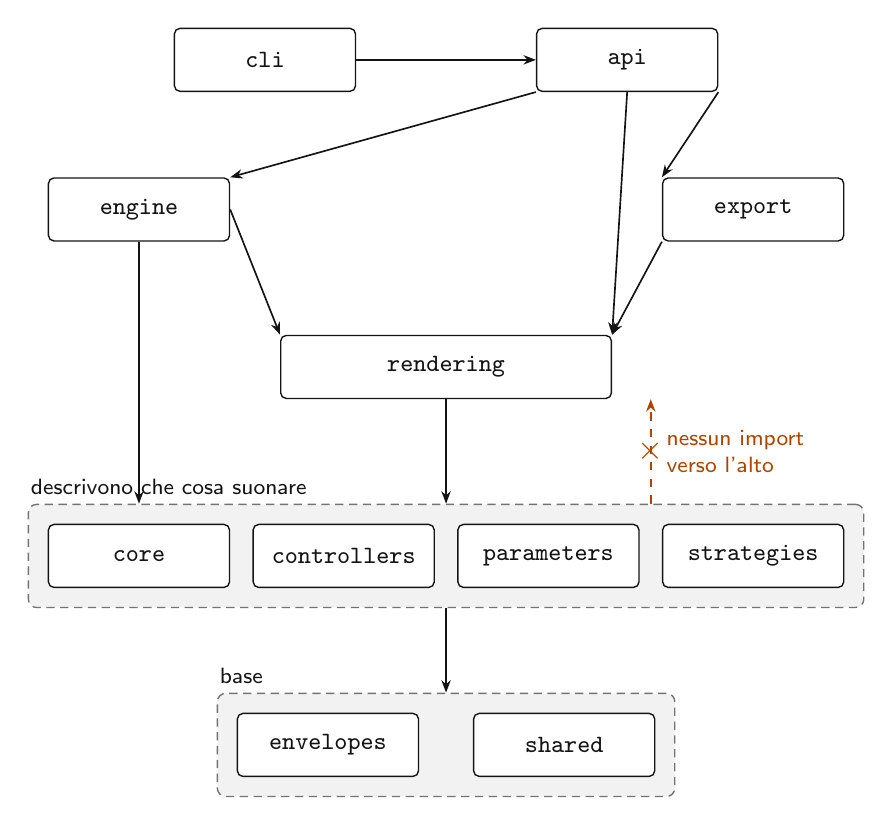
\begin{tikzpicture}[x=1cm,y=1cm]

% --- strati -----------------------------------------------------------------
\node[pkg] (cli) at (-2.3, 0)    {\texttt{cli}};
\node[pkg] (api) at ( 2.3, 0)    {\texttt{api}};
\node[pkg] (eng) at (-3.9,-1.9)  {\texttt{engine}};
\node[pkg] (exp) at ( 3.9,-1.9)  {\texttt{export}};
\node[pkg, minimum width=4.2cm] (ren) at (0,-3.9) {\texttt{rendering}};

\node[pkg] (cor) at (-3.9,-6.3) {\texttt{core}};
\node[pkg] (ctl) at (-1.3,-6.3) {\texttt{controllers}};
\node[pkg] (par) at ( 1.3,-6.3) {\texttt{parameters}};
\node[pkg] (str) at ( 3.9,-6.3) {\texttt{strategies}};
\begin{scope}[on background layer]
  \node[gruppo, fit=(cor)(ctl)(par)(str)] (gen) {};
\end{scope}
\node[etichetta] at (gen.north west) {descrivono che cosa suonare};

\node[pkg] (env) at (-1.5,-8.7) {\texttt{envelopes}};
\node[pkg] (sha) at ( 1.5,-8.7) {\texttt{shared}};
\begin{scope}[on background layer]
  \node[gruppo, fit=(env)(sha)] (base) {};
\end{scope}
\node[etichetta] at (base.north west) {base};

% --- dipendenze (chi importa chi) -------------------------------------------
\draw[dip] (cli) -- (api);
\draw[dip] (api.south west) -- (eng.north east);
\draw[dip] (api.south east) -- (exp.north west);
\draw[dip] (api.south) -- (ren.north east);
\draw[dip] (eng.east) -- (ren.north west);
\draw[dip] (exp.south west) -- (ren.north east);
\draw[dip] (eng.south) -- (eng.south |- gen.north);
\draw[dip] (ren.south) -- (ren.south |- gen.north);
\draw[dip] (gen.south) -- (gen.south |- base.north);

% --- l'import che non esiste ------------------------------------------------
\draw[mai] ([xshift=2.6cm]gen.north) -- ([xshift=2.6cm]ren.south)
      node[midway, right=2pt, text=vietato, font=\footnotesize, align=left] {nessun import\\verso l'alto};
\node[text=vietato, font=\large\bfseries] at ([xshift=2.6cm]$(ren.south)!0.5!(gen.north)$) {$\times$};

\end{tikzpicture}
\end{document}
